
\section*{Project Overview}
The Vulnerability Scanner project aims to develop a tool that identifies security vulnerabilities in software projects. It provides users with the ability to log in, create and manage projects, and scan code repositories or Python source files for various vulnerabilities. The system employs machine learning models to detect vulnerabilities and generates comprehensive reports. Users can rescan their code after making fixes to ensure security improvements.

\section*{Functional Requirements}
\begin{enumerate}
    \item \textbf{User Authentication}
    \begin{itemize}
        \item \textbf{Function:} Login with username and password
        \item \textbf{Description:} Users must authenticate themselves using a username and password to access the system. This ensures that only authorized users can utilize the scanner.
    \end{itemize}
    \item \textbf{Project Creation}
    \begin{itemize}
        \item \textbf{Function:} Create project
        \item \textbf{Description:} Users can create a new project by providing a name and selecting either a code repository (e.g., GitHub, Bitbucket) or uploading a Python source code file.
    \end{itemize}
    \item \textbf{Repository Management}
    \begin{itemize}
        \item \textbf{Function:} Choose repository or Python source code file
        \item \textbf{Description:} Users can specify the source of the code to be scanned. This can be a link to a repository or a direct upload of a Python source code file.
    \end{itemize}
    \item \textbf{Code Retrieval}
    \begin{itemize}
        \item \textbf{Function:} System will pull the repository
        \item \textbf{Description:} The system will fetch the code from the specified repository or process the uploaded Python source code file.
    \end{itemize}
    \item \textbf{Data Conversion}
    \begin{itemize}
        \item \textbf{Function:} System will convert it to w2v
        \item \textbf{Description:} The retrieved code will be converted to word2vec (w2v) format, preparing it for vulnerability analysis.
    \end{itemize}
    \item \textbf{Vulnerability Detection}
    \begin{itemize}
        \item \textbf{Function:} Find the vulnerability with one of the trained models (LSTM, CNN, MLP)
        \item \textbf{Description:} The system will analyze the word2vec formatted code using one of the pre-trained machine learning models: LSTM (Long Short-Term Memory), CNN (Convolutional Neural Network), or MLP (Multi-Layer Perceptron) to identify vulnerabilities.
    \end{itemize}
    \item \textbf{Report Generation}
    \begin{itemize}
        \item \textbf{Function:} System will generate report
        \item \textbf{Description:} After scanning, the system generates a detailed report outlining the detected vulnerabilities, their severity, and recommendations for fixing them.
    \end{itemize}
    \item \textbf{Rescan Capability}
    \begin{itemize}
        \item \textbf{Function:} User can rescan after fixes
        \item \textbf{Description:} Users can rescan their code after making the recommended fixes to ensure that vulnerabilities have been addressed.
    \end{itemize}
    \item \textbf{Supported Vulnerabilities}
    \begin{itemize}
        \item \textbf{Function:} System support the below vulnerabilities
        \item \textbf{Description:} The system specifically scans for the following types of vulnerabilities:
        \begin{itemize}
            \item XSS (Cross-Site Scripting)
            \item Path Disclosure
            \item Remote Code Execution
            \item Command Injection
        \end{itemize}
    \end{itemize}
\end{enumerate}

\section*{Technical Architecture}
\subsection*{System Components}
\begin{enumerate}
    \item \textbf{User Interface (UI):}
    \begin{itemize}
        \item Login Page
        \item Dashboard for project management
        \item Report viewing and rescan options
    \end{itemize}
    \item \textbf{Backend:}
    \begin{itemize}
        \item Authentication Service
        \item Project Management Service
        \item Code Retrieval Service
        \item Vulnerability Detection Service
        \item Report Generation Service
    \end{itemize}
    \item \textbf{Database:}
    \begin{itemize}
        \item User credentials
        \item Project details
        \item Scanning results and reports
    \end{itemize}
    \item \textbf{Machine Learning Models:}
    \begin{itemize}
        \item Pre-trained LSTM, CNN, and MLP models for vulnerability detection
    \end{itemize}
\end{enumerate}

\section*{Workflow}
\begin{enumerate}
    \item Login: User logs in using credentials.
    \item Project Creation: User creates a new project and selects the source of the code.
    \item Code Retrieval: System fetches the code from the repository or processes the uploaded file.
    \item Data Conversion: Code is converted to w2v format.
    \item Vulnerability Detection: Selected ML model analyzes the code for vulnerabilities.
    \item Report Generation: System generates and displays a report.
    \item Rescan: User can rescan the code after making fixes.
\end{enumerate}

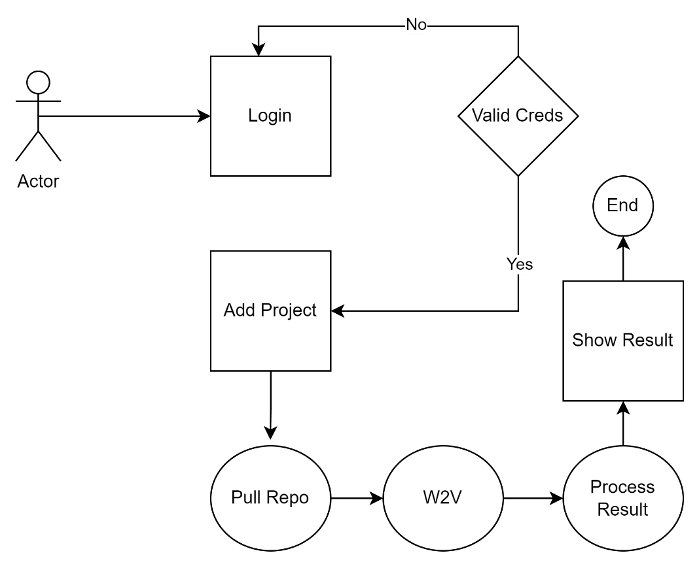
\includegraphics[width=0.9\textwidth]{pictures/workflow.png}

\section*{User Roles}
\subsection*{Administrator}
\begin{itemize}
    \item Manage users
    \item Oversee project activities
    \item View all generated reports
\end{itemize}

\subsection*{Regular User}
\begin{itemize}
    \item Create and manage their own projects
    \item Perform scans and view reports
    \item Rescan projects after fixes
\end{itemize}

\section*{Non-Functional Requirements}
\begin{itemize}
    \item \textbf{Security:} Ensure secure handling of user credentials and project data.
    \item \textbf{Performance:} Efficiently handle code retrieval and scanning for large repositories.
    \item \textbf{Scalability:} Support multiple concurrent users and scans.
    \item \textbf{Usability:} Provide an intuitive user interface for easy navigation and use.
\end{itemize}

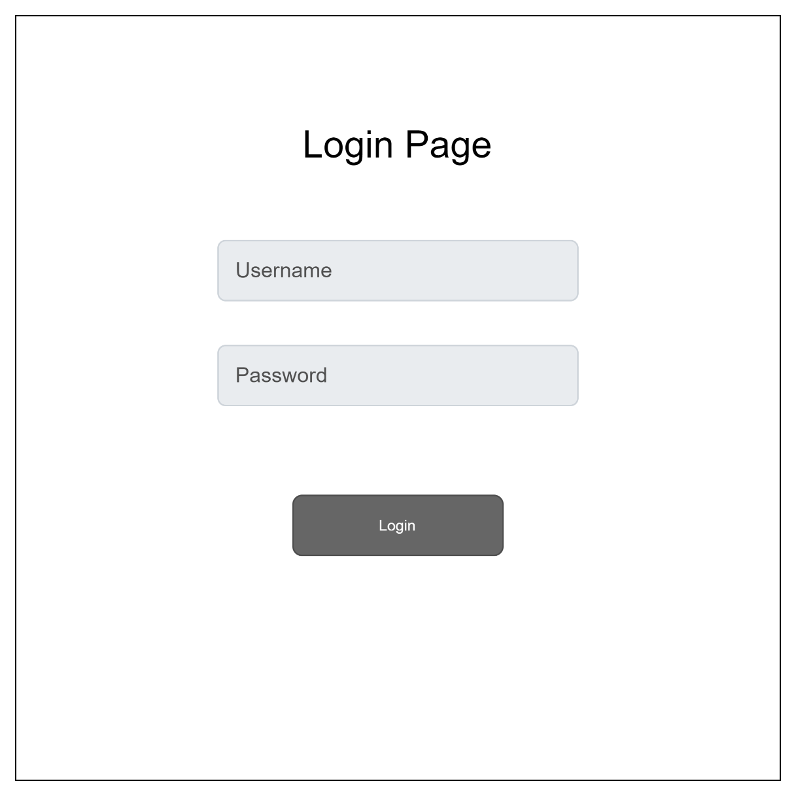
\includegraphics[width=0.9\textwidth]{pictures/loginPAge.png}
\newline
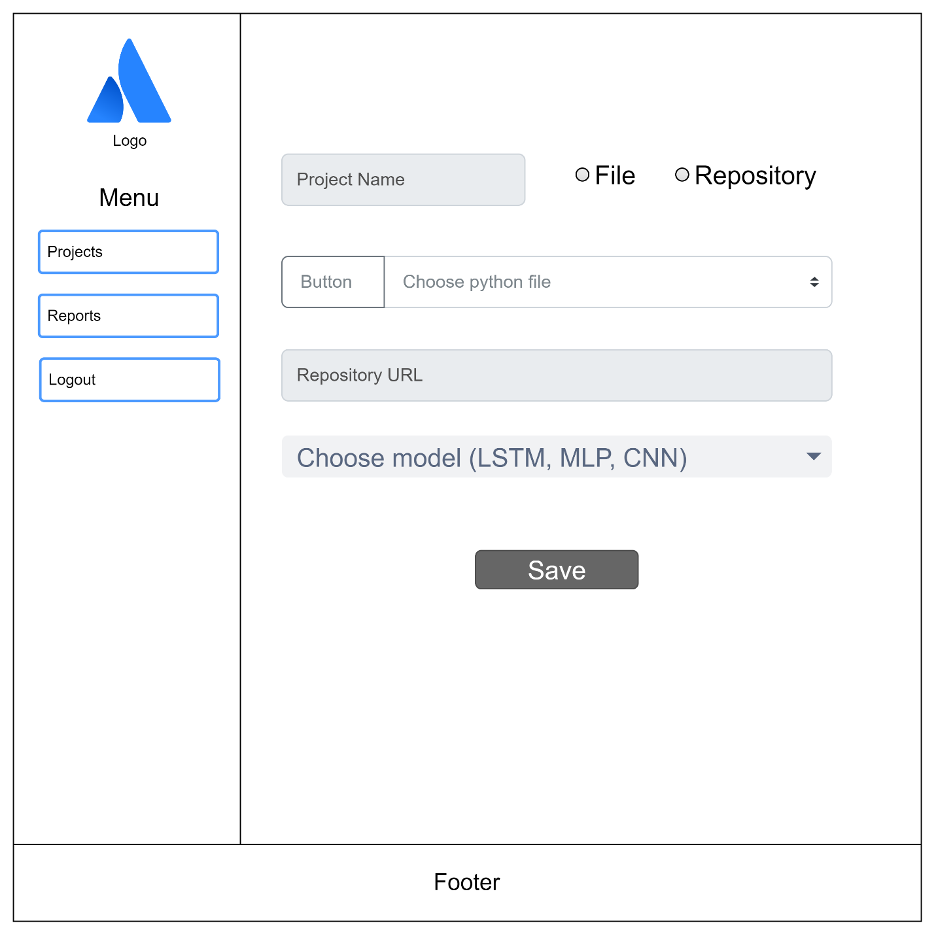
\includegraphics[width=0.9\textwidth]{pictures/menu.png}

\section*{Conclusion}
The Vulnerability Scanner project aims to provide a robust tool for identifying and fixing security vulnerabilities in software projects. By leveraging machine learning models, it ensures accurate and efficient vulnerability detection, aiding developers in maintaining secure codebases.

